\section{Hello Protocol}
\label{sec:hello-protocol}

The Hello Protocol module periodically sends Hello Interests to learn the activity status of the router's neighbors.
Hello Interests' names are constructed in the form: \texttt{/<neighbor's-router-prefix>/NLSR/INFO/<this-router's-prefix>}.
If a neighbor responds to a Hello Interest, the neighbor is considered to be up and \texttt{ACTIVE}.
A Hello Data's name is constructed using the following convention: \texttt{/<neighbor's-router-prefix>/NLSR/INFO/<this-router's-prefix>/<version>}.
If a neighbor fails to respond to a configurable number of Hello Interests (\texttt{hello-retries}), the neighbors is considered to be down and \texttt{INACTIVE}.
The Hello Protocol continues to send these periodic Hello Interests to each of its neighbors every \texttt{hello-interval} seconds.
If the Hello Protocol detects a change in a neighbors status
(i.e. a router that was previously \texttt{ACTIVE} is not responding to Hello Interests or a router that was previously \texttt{INACTIVE} responds to a Hello Interest),
it will notify the LSDB (Section~\ref{sec:lsdb}) to schedule a new Adjacency LSA build to include the updated neighbor information.

\subsection{Determining Neighbor's Status}
\label{sec:initial-status}

\begin{figure}
\center
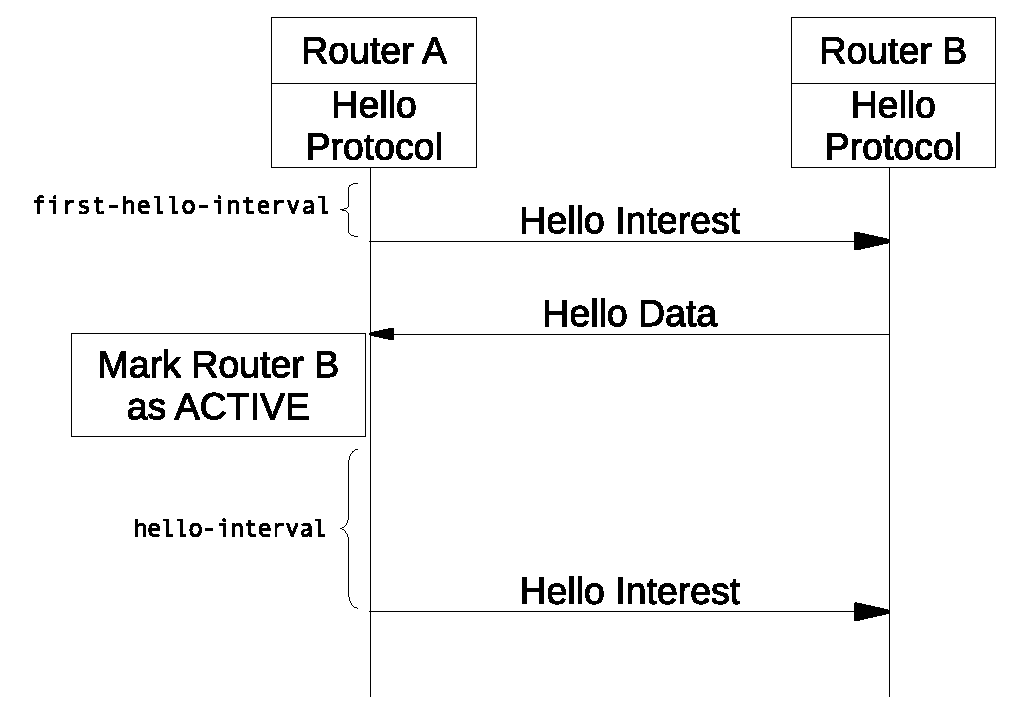
\includegraphics[width=0.5\textwidth]{figures/hello-protocol}
\caption{Router A determines the initial status of Router B}
\end{figure}

The Hello Protocol begins by scheduling Hello Interests to be sent to each neighbor of the router after \texttt{first-hello-interval} seconds.
When the scheduled event is triggered, the Hello Protocol iterates through the list of neighbors first checking if there is already a Face to the neighbor.
If there is a Face that has already been created, the Hello Protocol will construct and send a Hello Interest to the neighbor.
If a Face has not been created for the neighbor, the Hello Protocol will attempt to create a Face to the neighbor and register the neighbor's router prefix.
If the Face is created successfully, the Hello Protocol registers the Sync prefix, LSA prefix, and Key prefix using the Face ID returned by the Face creation command and sends out the Hello Interest.
If the Face cannot be created, the Hello Protocol considers the failure as a Hello Interest timeout.

If the Hello Protocol receives Data in response to the Hello Interest, it will first verify that the Data is signed by the correct entity.
If the Data is valid, the corresponding neighbor is set as \texttt{ACTIVE} and its timeout count is reset to zero.
If the neighbor was previously \texttt{INACTIVE}, an Adjacency LSA build is scheduled to include the newly \texttt{ACTIVE} neighbor.
If the Data is not valid, the packet is dropped.

If the Hello Interest sent to the neighbor times out, the corresponding neighbor's timed-out count is incremented.
If the neighbor's timed-out count is less than \texttt{hello-retries} in the configuration file, the Hello Protocol will send another Hello Interest after \texttt{hello-timeout} seconds.
If the neighbor's timed-out count equals the \texttt{hello-retries} value and the neighbor is currently marked as \texttt{ACTIVE}, the neighbor's status is set to \texttt{INACTIVE} and an Adjacency LSA build is scheduled. 

\subsection{Responding to Hello Interests}
\label{sec:respond-to-hello}

If the Hello Protocol receives a Hello Interest from another router, it will first verify that the Hello Interest came from one of its configured neighbors.
If so, the Hello Protocol responds to the Interest with Hello Data.
To optimize the time to respond to link recoveries, the Hello Protocol will then immediately send a Hello Interest to the neighbor if the neighbor is currently marked as \texttt{INACTIVE}.

\subsection{Failure and Recovery Detection}
\label{sec:link-failure}

\begin{figure}
\center
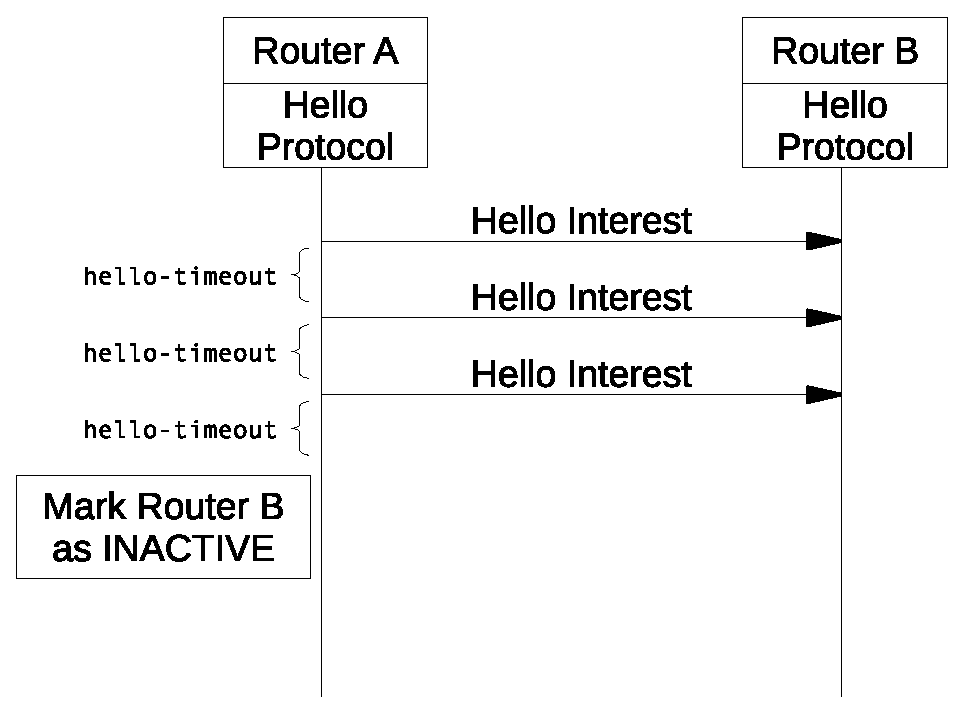
\includegraphics[width=0.5\textwidth]{figures/hello-protocol-timeout}
\caption{Router A determines that Router B has failed}
\end{figure}

The Hello Protocol will consider a neighbor as failed if the neighbor is currently \texttt{ACTIVE}, but Hello Interests sent to the neighbor have timed-out \texttt{hello-retries} number of times.
A failure can also be detected if a FaceEventNotification is received with the information that a Face to the neighbor has been destroyed.
The event is handled by the \texttt{Nlsr} class, but the triggered events simulate the actions of the Hello Protocol.
If the neighbor was currently \texttt{ACTIVE}, the neighbor will be set to \texttt{INACTIVE}, the neighbor's timed-out count will be set to \texttt{hello-retries}, and an Adjacency LSA build will be scheduled.

The Hello Protocol will consider a neighbor as recovered if the neighbor is currently \texttt{INACTIVE}, but the Hello Protocol has received valid Data in response to a Hello Interest sent to the neighbor.
